\section{Set up ANTLR}

Our first step will be to install and set up a \emph{parser generator}.
Nowadays, \emph{no one} really writes a complex parser completely by hand.
Although this is sometimes still necessary\footnote{Some languages are syntactically quite challenging.} most parsers can be whipped up pretty quickly using context-free \emph{string grammars}\footnote{For simple cases, \emph{regular expressions} can also be used.} typically in EBNF\footnote{Extended Backus-Naur Form}.
ANTLR~\cite{ANTLR} is a tool that can generate a parser from a compact EBNF specification for a host of target programming languages, including Java.
Although ANTLR might not be the most efficient or powerful parser generator out there, it is open-source, well documented and supported, and allows for a pragmatic and quite elegant \emph{fallback} to Java when things get nasty and we have to resort to some dirty tricks.

\begin{enumerate}
\item[$\blacktriangleright$] Install the ANTLR-IDE\footnote{\url{http://antlrv3ide.sourceforge.net/}} Eclipse plugin from:\\ \url{http://antlrv3ide.sourceforge.net/updates}.

We suggest you use ANTLR-IDE as it integrates nicely with eMoflon (the same build function for generating code also triggers the parser generator) and offers adequate editor functionality.

\item[$\blacktriangleright$] Download ANTLRWorks from:\\ \url{www.antlr.org/download/antlrworks-1.4.3.jar}.

ANTLRWorks\footnote{\url{http://www.antlr.org/works/index.html}} is the IDE recommended by \cite{ANTLR}.  
It offers a nice debugger and visualization of parse trees and abstract syntax trees.
You are free to use ANTLRWorks either together with ANTLR-IDE or as an alternative.
For all screenshots and explanations, however, we shall assume you choose to work with ANTLR-IDE.  

Now choose \texttt{Directory} and browse to the directory with the downloaded ANTLRWorks jar file (Fig.~\ref{moca-2-choose-path-to-jar}).

\item[$\blacktriangleright$] Configure ANTLR for Eclipse:\\ Go to ``Window/Preferences/ANTLR/Builder'' and choose \texttt{Add} as depicted in Fig.~\ref{moca-1-antlr-package}.

As ANTLR-IDE does not provide the actual jars for the parser generator, these have to be downloaded and referenced from the plugin.
%\usepackage{graphics} is needed for \includegraphics
\begin{figure}[!htbp]
\begin{center}
 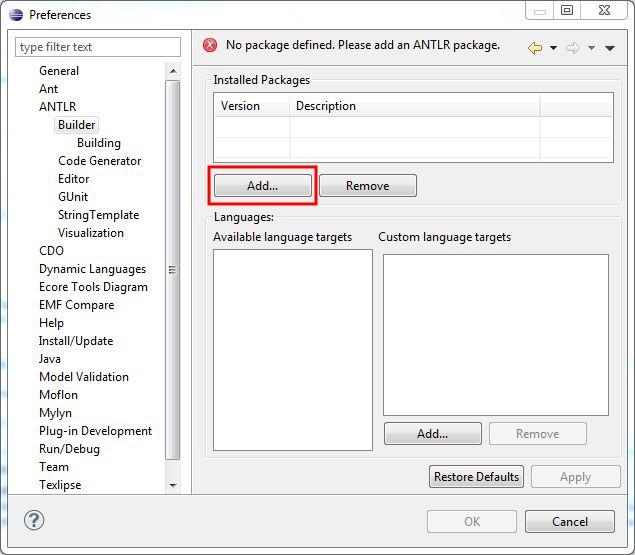
\includegraphics[width=0.8\textwidth]{pics/moca/0Install/1-antlr-package}
  \caption{Builder Preferences for ANTLR IDE}
  \label{moca-1-antlr-package}
\end{center}
\end{figure}
%\usepackage{graphics} is needed for \includegraphics
\begin{figure}[!htbp]
\begin{center}
 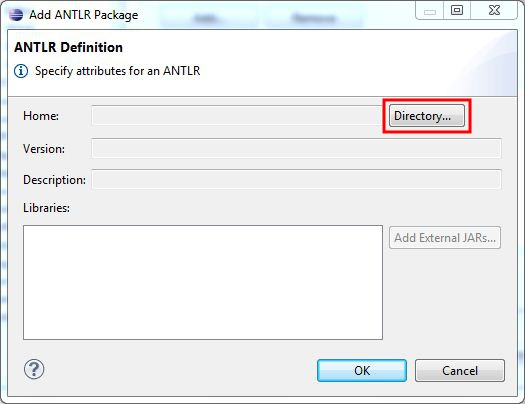
\includegraphics[width=0.8\textwidth]{pics/moca/0Install/2-choose-path-to-jar}
  \caption{Dialogue for choosing ANTLRWorks as Builder}
  \label{moca-2-choose-path-to-jar}
\end{center}
\end{figure}
\end{enumerate}

\clearpage